\documentclass[a4paper,14pt,russian]{extreport}
\usepackage[russian]{babel}

\usepackage{../common/dsturep_ru} % оформление по ДСТУ 3008-95
\usepackage{import}
\usepackage{standalone}
\usepackage{comment}
\usepackage{bbm}

\usepackage{tikz}
\usepackage{tikz-3dplot}
\usetikzlibrary{calc}
\usetikzlibrary{plotmarks}
\usepackage{pgfplots}

%\usepackage{scrextend}
\usepackage{changepage}
\usepackage{caption}
\usepackage{listings}
%\usepackage[title,titletoc]{appendix}
%\usepackage{appendix}
\usepackage{longtable}
%\usepackage{slashbox}
\usepackage{diagbox}
\usepackage{lscape}
\usepackage{algorithmic}
\usepackage{algorithm}

\def\male{male}
\def\female{female}

\bibliographystyle{../common/utf8gost780u}

\usepackage[square,numbers,sort&compress]{natbib}
\renewcommand{\bibnumfmt}[1]{#1.\hfill} % нумерация источников в самом списке — через точку

\def\passYear{2017}
\def\faculty{физико-технический институт}
\def\department{Кафедра информационной безопасности}
\def\departmentHead{Н. В. Грайворонский}
\def\kind{Дипломна робота}
\def\level{магістр}
\def\specialityCode{8.04030101}
\def\specialityTitle{Прикладная математика}
\def\theme{Решение нелинейных уравнений}
\def\gender{female}
\def\mentorGender{male}
\def\course{3}
\def\group{ФИ-41}
\def\name{Лавягина Ольга Алексеевна}
\def\mentorRank{}
\def\mentorName{Стёпочкина Ирина Валерьевна}
\def\reviewerRank{Rank}
\def\reviewerName{Name}
\def\subject{Методы вычислений}



\begin{document}

\import{1_title/}{title.tex}

\clearpage

\pagenumbering{gobble}
%\import{3_abstract/}{main.tex}

\pagestyle{empty}
\thispagestyle{empty}
\tableofcontents

\clearpage
\pagenumbering{arabic}
\pagestyle{fancy}
\setcounter{page}{2}

\clearpage

\chapter{Исходная система}

Нужно найти собственные значения матрицы $A$ с помощью метода Данилевского.

Для варианта 8 матрица имеет вид
\begin{equation*}
A =
\begin{bmatrix}
    5.26 & 0.10 & 0.55 & 1.28 \\
    1.10 & 4.44 & 1.30 & 0.16 \\
    0.55 & 1.30 & 6.44 & 2.10 \\
    1.28 & 0.16 & 2.10 & 8.10 \\
\end{bmatrix},
\end{equation*}

\chapter{Матрицы $M_i$ и $M_i^{-1}$}

\lstset{inputencoding=utf8, extendedchars=\true}
\lstinputlisting[language=bash,
                 basicstyle=\ttfamily\scriptsize]{../code/matrices}

\chapter{Результирующая матрица в форме Фробениуса}

\lstset{inputencoding=utf8, extendedchars=\true}
\lstinputlisting[language=bash,
                 basicstyle=\ttfamily\scriptsize]{../code/frobenius}

\chapter{Полученное характеристическое уравнение}

Характеристический полином строется раскрытием характеристического определителя матрицы
$P = M_1^{-1} M_2^{-1} M_3^{-1} AM_3 M_2 M_1$ по первой строке.
Он, вследствие подобия матриц $A$ и $P$, является так же и характеристическим полиномом матрицы $A$.

Раскрываем по первому столбцу
$$p \left( \lambda \right) =
  \left( -1 \right)^3 \cdot
  \left(
    \lambda^4 - 24.24 \lambda^3 + 208.3799 \lambda^2 - 761.624474 \lambda + 1003.73945
  \right).$$

\chapter{Собственные числа}

Собственные числа были найдены из уравнения $P \left( \lambda \right) = 0$.
Уравнение имеет 4 действительных корня (рис. \ref{fig:roots}):
$$ \lambda_1 = 3.57273, \,
  \lambda_2 = 4.97342, \,
  \lambda_3 = 5.59192, \,
  \lambda_4 = 10.1019.$$

\begin{figure}[h!]
  \centering
  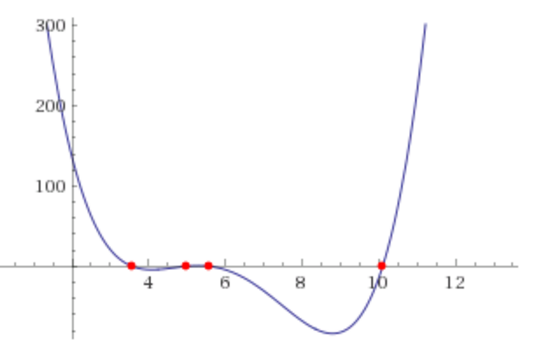
\includegraphics[width=.4\textwidth]{../code/roots.png}
  \caption{График корней}
  \label{fig:roots}
\end{figure}

\chapter{Листинг программы}

Листинг файла \_\_main\_\_.py
\lstset{inputencoding=utf8, extendedchars=\true}
\lstinputlisting[language=python,
                 basicstyle=\ttfamily\scriptsize]{../code/__main__.py}

Листинг файла solve.py
\lstset{inputencoding=utf8, extendedchars=\true}
\lstinputlisting[language=python,
                basicstyle=\ttfamily\scriptsize]{../code/solve.py}

\chapter{Проверка полученных результатов в WolframAlpha}

Была использована функция eigenvalues и получены такие результаты (рис. \ref{fig:wolfram}):
$$ \lambda_1 = 10.1019, \,
  \lambda_2 = 5.59192, \,
  \lambda_3 = 4.97342, \,
  \lambda_4 = 2.57273.$$

\begin{figure}[h!]
  \centering
  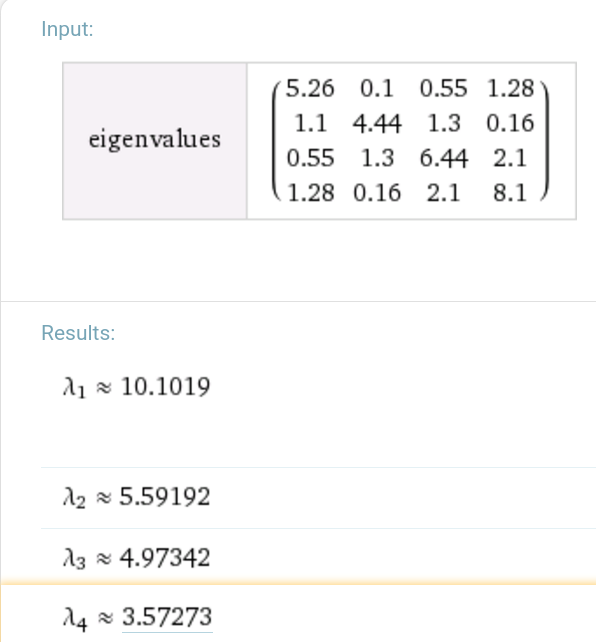
\includegraphics[width=.4\textwidth]{../code/wolframalpha_result.png}
  \caption{Проверка полученных результатов в WolframAlpha}
  \label{fig:wolfram}
\end{figure}

\chapter*{Выводы}
\addcontentsline{toc}{chapter}{Выводы}

Собственные числа матрицы были найдены с помощью метода Данилевского.
Для этого исходная матрица $A$ была преобразована так,
что она имеет ненулевые элементы только в первой строке,
и элементы на смещённой диагонали равны единице, то есть матрица приведена к форме Фробениуса.

Найдены собственные числа матрицы с помощью WolframAlpha.
Полученные решения полностью совпадают.

\end{document}
